\section {Inovação Social}
\label{inovacaosocial}

Como visto na seção anterior, o conceito de Inovação de Schumpeter trata das atividades inventivas para novos processos, produtos e serviços, visando principalmente a maximização de lucro. 

Já a Inovação Social, é voltada para a criação de métodos, processos e difusões de novas ideias para a resolução de problemas que atendam as necessidades sociais e que fortaleçam autonomia de gestão das próprias organizações. \cite{monteiro2019}

A inovação social surge em decorrência das soluções propostas pelo mercado para problemas sociais se mostrarem ineficazes por não atuarem no cerne dos problemas da comunidade. Em decorrência disto, essas tarefas acabam recaindo sobre o estado, que também não se mostra eficaz, por reforçar os modelos antigos de inovação, ao invés de novos modelos, e sobre a própria sociedade civil. \cite{murray2010}

\citeauthor{murray2010} (\citeyear{murray2010}, p. 11-13) propõe um modelo espiral de seis etapas, sistematizando a realização da Inovação Social:

\begin{figure}[H]
    \caption{Modelo espiral de Inovação Social}
    \centering
    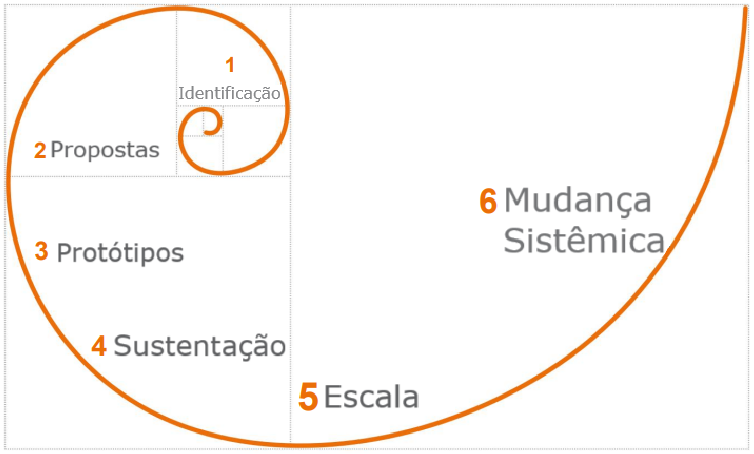
\includegraphics[width=\linewidth]{images/fundamentacao/modelomurray.png}
    \label{fig:modelomurray}
    
    Fonte: Adaptado de \citeauthor{murray2010} (\citeyear{murray2010}, p. 11).
\end{figure}

\begin{itemize}
    \item \textbf{Identificação, inspirações e diagnósticos}: essa primeira etapa é a identificação das questões que demonstram a necessidade da inovação, por um panorama de situações como: crises, falta de orçamento, baixo desempenho. Também trata das inspirações que podem ser utilizadas para auxiliar a alavancar a organização. O diagnóstico busca encontrar de fato a raiz daquilo que está originando os problemas identificados no início da etapa;
    \item \textbf{Propostas e ideias}: nessa fase serão geradas as ideias para a solução dos problemas elencados na etapa de Identificação, inspirações e Diagnósticos. Nessa etapa, podem ser utilizadas metodologias já existentes, como, por exemplo, as que são utilizadas no \textit{Design Thinking}, que irão facilitar a ideação, por serem metodologias já testadas, conhecidas e validadas. Essa etapa visa extrair percepções que podem fazer parte da implementação das soluções inovativas posteriormente;
    \item \textbf{Prototipagem e pilotos}: nessa etapa as ideias começam a sair do papel. Podem ser utilizadas metodologias já existentes como por exemplo \textit{Wireframe}, prototipação por \textit{mockups}, dentre outras. É necessária a participação dos autores nesse processo de experimentação, pois o processo de refinamento da solução deve passar por todos que irão utilizá-la, visando reduzir erros e conflitos, pois diferentes interesses dos usuários surgirão ao longo da prototipagem da solução. Também serão delimitadas as métricas necessárias para o êxito da solução;
    \item \textbf{Sustentação}: depois do protótipo pronto, é necessário aprimorar as ideias e os fluxos que irão garantir a sustentação financeira da solução pensada e concebida nas etapas anteriores, identificando: questões orçamentárias necessárias, equipe de criação, implantação e manutenção da solução, legislação vigente, dentre outras questões pertinentes. Uma solução que não consegue ter sua sustentação a longo prazo, pode acabar sendo descontinuada.
    \item \textbf{Escala e difusão}: após consolidada as questões necessárias para a sustentação e manutenção da ideia proposta, agora é necessário existir um planejamento de escalabilidade da mesma, pensando no crescimento e disseminação da inovação. Nesse ponto é necessário considerar tanto a oferta como a demanda, a exemplo da demanda do mercado, dos formuladores de políticas sociais, dentre outros, auxiliando a disseminação bem-sucedida da ideia proposta. Na inovação social esse crescimento pode ser aplicado de várias formas, como, por exemplo, fornecimento de suporte, competências e habilidades para outras ideias crescerem.
    \item \textbf{Mudança Sistêmica}: é o objetivo final da Inovação Social. Essa etapa envolve muitos elementos necessários para as mudanças propostas serem de fatos consolidadas: movimentos sociais, modelos de negócios, leis, dados, infraestruturas, e novas formas de pensar. As Inovações Sociais podem esbarrar em métodos antigos e burocráticos que tentarão engessar o processo inovativo. É fundamental a necessidade da transformação das estruturas sociais e políticas, em resposta as inovações propostas.
\end{itemize}

Existe também outro processo para a prática da Inovação Social chamado de \textit{Speedplay}, proposto por Maria Angela Ferrario, direcionada a comunidades de difícil acesso pelo serviço público, com projetos com curto espaço de tempo para serem executados, com uma visão de que os artefatos desenvolvidos são veículos para a mudança social. Esse processo é aplicado em quatro etapas: \cite{ferrario2014}. 

\begin{figure}[H]
    \caption{Metodologia \textit{Speedplay}}
    \centering
    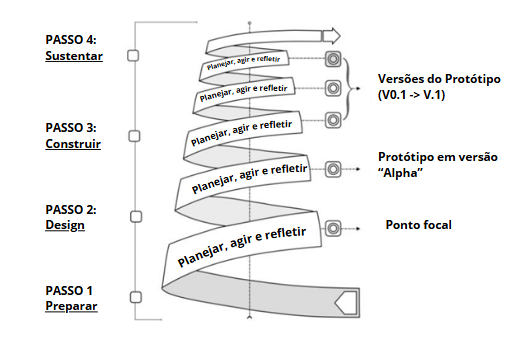
\includegraphics[width=\linewidth]{images/fundamentacao/speedplay.png}
    \label{fig:speedplay}
    
    Fonte: Adaptado de \citeauthor{ferrario2014} (\citeyear{ferrario2014}).
\end{figure}

\begin{itemize}
    \item \textbf{Passo 1 - Preparar:} construção de confiança do time e aprimoramento de habilidades e levantamento de requisitos via Pesquisa-Ação para compreensão das necessidades dos usuários e do contexto social. Nessa etapa existe um Ponto focal, um evento aberto ao público, visando a cocriação de um projeto de protótipo, visando estimular o ritmo e a participação dos envolvidos;
    \item \textbf{Passo 2 - Design:} refinamento dos requisitos dos usuários e cocriação de um possível protótipo utilizando Design Participativo;
    \item \textbf{Passo 3 - Construir:} construção de protótipo e desenvolvimento do sistema iterativamente, validando com os usuários, via metodologias ágeis;
    \item \textbf{Passo 4 - Sustentar:} planejamento do suporte ao desenvolvimento futuro do sistema, busca de parcerias para tal, além do compartilhamento das lições aprendidas e do entendimento técnico do sistema.
\end{itemize}

Apesar dos dois processos tratarem da prática da Inovação Social, existem diferenças fundamentais na concepção da aplicabilidade de cada uma das metodologias. O modelo espiral de Inovação Social de \citeauthor{murray2010} (\citeyear{murray2010}) é um modelo composto por seis etapas na sua execução, sendo direcionado para qualquer tipo de Inovação Social, e seus prazos de execução são mais longos. Já o modelo \textit{Speedplay} de \citeauthor{ferrario2014} (\citeyear{ferrario2014}) é um modelo que utiliza metodologias ágeis, sendo pensado para a concepção de artefatos, já que algumas de suas etapas são focados na construção de protótipos, com prazos de execução mais curtos. Caberá aos decisores das organizações sociais decidirem qual das metodologias de Inovação Social se encaixará melhor na realidade da organização em que será aplicado.

Existem outros modelos para auxiliar na prática da Inovação Social Aberta, porém, estes citados anteriormente são os mais comuns na área da Inovação Social praticada para a área da Computação.

